\documentclass[../distribution_theory_notes.tex]{subfiles}
\begin{document}
\section{Aula 02 - 19 de Agosto, 2024}
\subsection{Motivações}
\begin{itemize}
	\item Espaços de Fréchet;
	\item Seminormas.
\end{itemize}
\subsection{Espaços de Fréchet}
Podemos dizer que a Teoria das Distribuições é uma parte da análise funcional que se desenvolve separadamente dos espaços de Banach ou de Hilbert, tendo em vista que ela examina espaços duais de certos espaços vetoriais de funções, as chamadas funções ``testes'', cuja maneira natural de convergência é uma que não pode ser descrita por uma norma, mas que, felizmente, ainda é compatível com a estrutura linear dos mesmos, que nos leva ao conceito dos Espaços Vetoriais Topológicos. 

Mesmo não sendo normados, eles possuem algumas propriedades análogas às do espaço normado que são úteis para a obtenção das propriedades que desejamos, tais como: 
\begin{itemize}
  \item[i)] Metrizabilidade: permite o estudo por meio de limites de sequências;
  \item[ii)] Convexidade Local: as bolas, tanto abertas quanto fechadas, são convexas;
  \item[iii)] Possui SFV equilibrado: a origem possui um SFV ``invariante por rotação escalar'' e simétrico com relação à origem; e 
  \item[iv)] Completeza: o que faz deles espaços de Baire, ou seja, isenta a análise da consideração de ``conjuntos insignificantes''. 
\end{itemize}
A classe de TVS que cumpre todos os requisitos acima listados e não necessariamente normado é chamada de \textbf{Espaços de Fréchet}; trataremos deles na aula de hoje.

\begin{theorem*}
  Em um TVS \((E, \tau )\), toda vizinhança U da origem contém uma vizinhança equilibrada da origem.
\end{theorem*}
\begin{proof*}
  Com efeito, como \(M(0, 0)=0 \cdot 0 = 0\in U\), segue da continuidade da multiplicação que existem \(\delta > 0\) e \(V\in \tau \), com \(0\in V\) tais que \(B_{\mathbb{C}}(0; \delta )\times V\subseteq M^{-1}(0)\), ou seja, 
    \[
      |\lambda |<\delta \;\&\; x\in V \Rightarrow \lambda \cdot x\in U.
    \]
    Daí, segue que 
      \[
        B\coloneqq \bigcup_{|\lambda |<\delta }^{}\lambda \cdot V=M(B_{\mathbb{C}}(0; \delta ) \times V) \subseteq U
      \]
      e que B é equilibrado, já que, se \(|\alpha |\leq 1,\; |\alpha \lambda |\leq |\lambda |<\delta \) , então \((\alpha \lambda )V\) está contido em B, isto é, 
        \[
          |\alpha |\leq 1 \Rightarrow \alpha B \subseteq B.
        \] 
 \begin{figure}[H]
 \begin{center}
 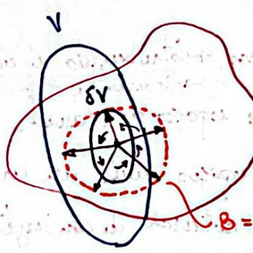
\includegraphics[height=0.5\textheight, width=0.5\textwidth, keepaspectratio]{./Images/open_union_2.png}
 \end{center}
 \caption{o conjunto B é a reunião de todas as rotações de \(\delta V\) ao redor da origem, deixando-o ``redondo''.}
 \end{figure} 

  Finalmente, que B é vizinhança da origem segue do fato de que B é a reunião de abertos: 
    \[
      B = \bigcup_{0<|\lambda |<\delta }^{}\lambda V,
    \]
    conforme o segundo item do Lema 1. 
\end{proof*}
\begin{theorem*}
  Toda vizinhança conexa U da origem de um TVS \((E, \tau )\) contém uma vizinhança da origem convexa e equilibrada.
\end{theorem*}
\begin{proof*}
  Com efeito, primeiramente consideremos uma vizinhança equilibrada da origem B contida em U e notemos que, para \(|\lambda |=1\), tem-se \(\lambda B = B.\) Com isso, se 
    \[
      C\coloneqq \bigcap_{|\lambda |=1}^{}\lambda \cdot U,
    \]
    então, como intersecção de convexos, C é convexo e 
      \[
        B = \lambda B\subseteq \lambda U,\quad \forall |\lambda |=1,
      \] 
      donde segue que B está contido em C, mostrando que o interior de C é não vazio; desta forma, pondo \(V\coloneqq \mathrm{int}(C)\), afirmamos que este é o conjunto do teorema. 

      De fato, V é vizinhança da origem, pois 
        \[
          0\in B\subseteq \mathrm{int}(C)=V;
        \]
        além disso, V é convexo, pois o interior de um convexo é um convexo. Por fim, como U é convexo e 0 pertence a ele, para \(0\leq t\leq 1\) e x em U, tem-se que 
          \[
            tx + (1-t)0\in U,
          \]
          isto é, para \(0\leq t\leq 1\), 
            \[
              tU\subseteq U;
            \]
            logo, dado \(|\alpha |\leq 1\), como \(\alpha =|\alpha |e^{i\theta }\), concluímos que 
              \[
                \alpha C = \bigcap_{|\lambda |=1}^{}(e^{i\theta }\lambda )|\alpha |U = \bigcap_{|\alpha |=1}^{}|\alpha | U \subseteq \bigcap_{|\alpha |=1}^{}U = C.
              \]
              Portanto, C é equilibrado, fazendo com que V, como interior de um conjunto equilibrado, também o seja. \qedsymbol

\end{proof*}

  \begin{tcolorbox}[
  skin=enhanced,
  title=Lembrete!,
  after title={\hfill Interior de Convexo},
  fonttitle=\bfseries,
  sharp corners=downhill,
colframe=black,
  colbacktitle=yellow!75!white, 
  colback=yellow!30,
  colbacklower=black,
coltitle=black,
  %drop fuzzy shadow,
  drop large lifted shadow
  ]
  Para D convexo, tem-se 
    \[
      M_t(\mathrm{int}(D))=\mathrm{int}(M_t(D))\;\text{ou}\; \mathrm{int}(tD)=t \mathrm{int}(D)\in \tau_{E},\; t\neq 0.
    \] 
    Assim, 
      \[
        (1-t)D + tD\subseteq D \Rightarrow (1-t)\mathrm{int}(D)+t \mathrm{int}(D) \subseteq (1-t)D + tD \subseteq D,
      \]
      e, sendo o conjunto à esquerda um aberto, segue que ele está contido no interior de D.
  \end{tcolorbox}

  Uma consequência do teorema acima é que, em qualquer TVS, a origem possui um SFV equilibradas e, se ela possui um SFV convexas, então ele possui um SFV convexas E equilibradas.

  \begin{def*}
    Um TVS \((E,  \tau )\) se diz \textbf{localmente convexo} quando a origem possui um SFV convexas (portanto convexas, equilibradas e absorventes). \(\square\)
  \end{def*}
 \begin{example}
   Se \((E, \Vert \cdot  \Vert_{E})\) é normado, então \(\mathcal{B}\coloneqq \{B(0; 1/n):\; n\in \mathbb{N}\}\) é um SFV da origem formado por convexos e enumerável; por outro lado, para \(0<p<1\), o espaço \(L^{p}(\mu )\) não é localmente convexo (pelo menos quando \(\mu \) é dx em \([0, 1]\))\footnote{Embora não provaremos isso neste curso, só há uma única maneira de introduzir topologias localmente convexas em um espaço vetorial, e é por meio de uma família de \textit{seminormas}.}. 
 \end{example}
\begin{def*}
  Uma \textbf{seminorma} em E, espaço vetorial, é uma função \(p:E\rightarrow \mathbb{R}\) tal que:
 \begin{align*}
   &(i)\; p(x+y)\leq p(x)+p(y),\quad \forall x, y\in I;\\ 
   &(ii)\; p(\lambda x)=|\lambda |p(x),\quad \forall x\in E\;\&\;\lambda \in \mathbb{C}.
 \end{align*}
 Se, além disso, a seminorma satisfaz 
   \[
     p(x)=0\Rightarrow x=0, 
   \]
   então  p é dita \textbf{norma em E}.
\end{def*}
\begin{figure}[H]
\begin{center}
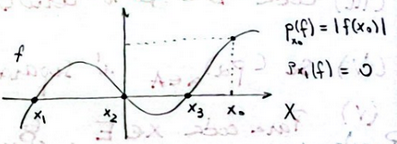
\includegraphics[height=0.5\textheight, width=0.5\textwidth, keepaspectratio]{./Images/seminorm_02.png}
\end{center}
\caption{enquanto as normas são nulas se, e só se, x em si é a origem, as seminormas podem se anular mesmo em valores distintos da origem. Assim, elas são ``medições'' parciais dos vetores, ao contrário das normas, que vêem os objetos globalmente.}
\end{figure}
\begin{def*}
  Uma família \(\{p_{\alpha }\}_{\alpha \in A}\) de seminormas em E se diz \textbf{separante} quando, para cada x não nulo, existir \(\alpha =\alpha_{x}\) em A tal que \(p_{\alpha }(x)\neq 0\). \(\square\)
\end{def*}
Uma forma de entender a definição acima é que uma só \(p_{\alpha }\) pode não ``enxergar'' o zero de E, mas toda a família sim, pois a condição equivale a 
  \[
    p_{\alpha }(x)=0,\; \forall \alpha \in A \Rightarrow x=0.
  \]

  Nosso próximo passo é construir uma topologia num espaço vetorial a partir de uma família de seminormas; porém, para isso, é preciso lembrar quais condições uma família \(\mathcal{B}\) de subconjuntos de X qualquer deve satisfazer para servir como base de uma topologia em X:
  \begin{theorem*}[Condições para Base]
    Uma família \(\mathcal{B}\) de subconjuntos de X é base de alguma topologia \(\tau \) em X se, e somente se, ela cumpre as seguintes condições: 
   \begin{itemize}
     \item[a)] Para cada x em X, existe um elemento da família \(B_{x}\in \mathcal{B}\) tal que \(x\in B_{x}\); e 
       \item[b)] Dados elementos \(B_1,\; B_2\) de \(\mathcal{B}\) e um ponto x comum a ambos, ou seja, \(x\in B_1\cap B_2\), então existe \(B_3\) em \(\mathcal{B}\) com 
       \[
       x\in B_3\subseteq B_1\cap B_2.
       \]
   \end{itemize}
  \end{theorem*}
 \begin{figure}[H]
 \begin{center}
 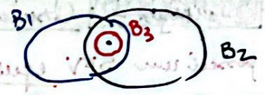
\includegraphics[height=0.5\textheight, width=0.5\textwidth, keepaspectratio]{./Images/basis_X_02.png}
 \end{center}
 \caption{a ideia é que, caso o ponto caia na intersecção de dois elementos da suposta base, é possível ``afunilar'' para um elemento individual dela ao invés de ficar trabalhando com a intersecção.}
 \end{figure}
 \begin{proof*}
   A prova consiste em definirmos 
     \[
       \tau \coloneqq \{\emptyset \}\cup \bigcup_{i\in I}^{}B_{i}, \quad B_{i}\in \mathcal{B},
     \]
     onde I é uma família arbitrária de índices. Portanto, \(\tau \) é uma topologia em X que admite \(\mathcal{B}\subseteq \tau \) como base. \qedsymbol
 \end{proof*}
\begin{example}
  A topologia produto, definida por uma família 
    \[
      \{f_{\alpha }:X\rightarrow (X_{\alpha }, \tau_{\alpha })\}_{\alpha \in A}
    \]
    é obtida a partir deste procedimento.
\end{example}
\begin{def*}
  Se \(\{p_{\alpha }\}_{\alpha \in A}\) é uma família de seminormas em E, x é um ponto dele e \(\varepsilon \) é um número positivo qualquer, definimos uma \textbf{semibola centrada em x com raio \(\varepsilon \)} como o conjunto 
    \[
      B_{\alpha }(x; \varepsilon )\coloneqq \{y\in E:\; p_{\alpha }(y-x)<\varepsilon \}. \quad \square
    \]
\end{def*}
\begin{prop*}
  Dada uma família \(\{p_{\alpha }\}_{\alpha \in A}\) de seminormas em E, para cada x em E, \(\alpha \) em A e \(\varepsilon \) positivo. Defina a família 
    \[
    \mathcal{B}\coloneqq \biggl\{\bigcap_{j=1}^{n}B_{\alpha_{j}}(x_{j}; \varepsilon_{j}):\;\alpha_{j}\in A,\; x_{j}\in E,\; \varepsilon_{j}>0,\; n\in \mathbb{N}\biggr\}
    \]
    de intersecções finitas de semibolas (pode ser o mesmo x para todo índice j e o mesmo \(\varepsilon \) positivo, mas a prova muda). Então, temos: 
   \begin{itemize}
     \item[i)] A família \(\mathcal{B}\) é a base de uma topologia \(\tau \) em E (de fato, a topologia mais fina que torna contínuas as funções \(p_{\alpha }:E\rightarrow \mathbb{R}\));
       \item[ii)] \(\tau \) é compatível com a estrutura linear de E; 
         \item[iii)] Cada membro B da família \(\mathcal{B}\) é convexo; 
         \item[iv)] Se \(\{p_{\alpha }\}_{\alpha \in A}\) é separante, então \(\tau \) é Hausdorff;
           \item[v)] Para cada x em E, a família 
             \[
             \mathcal{B}_{x}\coloneqq \biggl\{\bigcap_{j=1}^{n}B_{\alpha_{j}}(x; \varepsilon_{j}):\; \alpha_{j}\in A,\; \varepsilon_{j}>0,\; n\in \mathbb{N}\biggr\}
             \]
             é um SVF convexas de x; e 
           \item[vi)] Se A é enumerável e \(\{p_{\alpha }\}_{\alpha \in A}\) é separante, então \(\tau \) é enumerável (consequentemente, existe uma métrica d em E segundo a qual U é aberto com respeito a \(\tau \) se, e somente se, U é aberto com respeito a d).
   \end{itemize}
\end{prop*}
\begin{proof*}
  Por definição, \(\mathcal{B}\) satisfaz as condições do teorema anterior de caracterização de bases; logo, temos uma topologia em E que admite \(\mathcal{B}\) como base, dada por 
    \[
      \tau =\{\emptyset \}\cup \biggl\{\bigcup_{B\in \mathcal{A}}^{}B:\; \mathcal{A}\subseteq \mathcal{B}\biggr\},
    \]
    provando o primeiro item. 

    Dito isso, como, para todos x e y em E e \(0\leq t\leq 1\), as seminormas satisfazem 
      \[
        p_{\alpha }(tx + (1-t)y)\leq tp_{\alpha }(x)+ (1-t)p_{\alpha }(y),
      \]
      vale que cada \(B_{\alpha }(x; \varepsilon )\) é convexo; logo, cada B em \(\mathcal{B}\) é convexo, provando o item (iii).

      Com respeito a (iv), supondo que \(\{p_{\alpha }\}_{\alpha \in A}\) é separante, dados elemento x e y distintos, existe \(\alpha_{0}\) em A tal que podemos pôr
        \[
          \delta \coloneqq p_{\alpha_{0}}(x-y) >0.
        \]
        Consequentemente, 
          \[
            B_{\alpha_{0}}\biggl(x; \frac{\delta }{2}\biggr)\cap B_{\alpha_{0}}\biggl(y; \frac{\delta }{2}\biggr) = \emptyset 
          \]
          com ambas pertencentes à família \(\mathcal{B}\), mostrando que \(\tau \) é Hausdorff. 

          A prova do item (ii) começa com a adição: dados \(\mathfrak{A}(x_{0}, y_{0})=x_{0}+y_{0}\) em E e \(\varepsilon >0\), segue de 
            \[
              p_{\alpha }(\mathfrak{A}(x, y)-\mathfrak{A}(x_{0}, y_{0}))=p_{\alpha }((x-x_{0})+(y-y_{0}))\leq p_{\alpha }(x-x_{0})+p_{\alpha }(y-y_{0})
            \]
            que 
              \[
                B_{\alpha }\biggl(x_{0}; \frac{\varepsilon }{2}\biggr)\times B_{\alpha }\biggl(y; \frac{\varepsilon }{2}\biggr)\subseteq \mathfrak{A}^{-1}(B_{\alpha }(x_{0}+y_{0}; \varepsilon )),
              \]
              e isso é suficiente para mostrar a continuidade de \(\mathfrak{A}\) no ponto \((x_{0}, y_{0})\) de \(E\times E\), tendo em vista que o índice \(\alpha \) de A também foi arbitrário
              Agora, dados \(\lambda_{0}\) complexo, \(\alpha \) índice qualquer e um ponto \(x_{0}\) de E, temos 
             \begin{align*}
               p_{\alpha }(\mathfrak{M}(\lambda , x)-\mathfrak{M}(\lambda_{0}, x_{0})) &= p_{\alpha }(\lambda x - \lambda_{0}x_{0})\\ 
                                                                                       &=p_{\alpha }(\lambda x - \lambda x_{0} + \lambda x_{0} -\lambda_{0}x_{0})\\ 
                                                                                       &\leq |\lambda |p_{\alpha }(x-x_{0})+|\lambda -\lambda_{0}|p_{\alpha }(x_{0}),
             \end{align*}
             donde vemos que existem dois casos possíveis a serem considerados: 

             \textbf{\underline{Caso \(p_{\alpha }(x_{0})=0\)}:} dada uma semibola \(B_{\alpha }(\lambda_{0}x_{0}; \varepsilon )\), tomamos 
               \[
                 \Lambda \coloneqq |\lambda_{0}| + 1 > 0 \quad\&\quad \delta_{2}\coloneqq \frac{\varepsilon }{\Lambda }.
               \]
               Disso, segue que 
                 \[
                   |\lambda -\lambda_{0}|<1\;\&\; x\in B_{\alpha }(x_{0}; \delta_{2}) \Rightarrow \lambda x\in B_{\alpha }(\lambda_{0}x_{0}; \varepsilon ).
                 \]

                 \textbf{\underline{Caso \(p_{\alpha }(x_{0})>0\)}:} neste, tomamos 
                   \[
                     \delta_1\coloneqq \frac{\varepsilon }{2p_{\alpha }(x_{0})} \quad\&\quad \delta_{2}\coloneqq \frac{\varepsilon }{2(\delta_{1}+|\lambda_{0}|)}.
                   \]
                   Assim, temos 
                     \[
                       |\lambda -\lambda_{0}|<\delta_1 \;\&\; x\in B_{\alpha }(x_{0}; \delta_{2})\Rightarrow \lambda x\in B_{\alpha }(\lambda_{0}x_{0}; \varepsilon ).
                     \]
                    
                     Em ambos os casos, a continuidade da multiplicação por escalar foi garantida, consequentemente provando o item (ii)

                     Para a prova do item (vi), provaremos a Metrizabilidade de \(\tau \) ao supor A enumerável. Faremos apenas o caso em que A é enumerável; na verdade, supomos que \(A=\mathbb{N}.\) Assim, é suficiente mostrar que cada ``Bola'' \(B_{j}(x; \varepsilon )\) é aberta segundo d e que cada \(B_{d}(x; \varepsilon )\) é aberta segundo \(\tau \), onde 
                       \[
                         d(x, y)\coloneqq \sum\limits_{i=1}^{\infty}\frac{1}{2^{j}}\frac{p_{j}(x-y)}{1+p_{j}(x-y)}
                       \]
                       é a métrica invariante. Note que esta métrica está bem definida, tendo em vista que, para cada j natural, 
                         \[
                           0\leq \frac{p_{j}(z)}{1+p_{j}(z)}\leq 1
                         \]
                         e 
                           \[
                             \sum\limits_{j=1}^{\infty}\frac{1}{2^{j}}=1<\infty.
                           \]
                           Quanto ao fato dela ser uma métrica, ele segue de \(\{p_{j}\}_{j\in \mathbb{N}}\) ser separante e 
                             \[
                               \varphi (t)=\frac{t}{t+1}
                             \]
                             ser crescente para \(t\geq c\) (Verifique!).

                             Agora, seja \(\tau_{d}\) a topologia induzida por d. Por um lado, como, para cada n natural, 
                               \[
                                 d(x, y)=\sum\limits_{j=1}^{N}\frac{1}{2^{j}}\frac{p_{j}(x-y)}{1+p_{j}(x-y)} + \sum\limits_{j=N+1}^{\infty}\frac{1}{2^{j}}\frac{p_{j}(x-y)}{1+p_{j}(x-y)} \leq \sum\limits_{j=1}^{N}p_{j}(x-y)+\sum\limits_{j=N+1}^{\infty}\frac{1}{2^j},
                               \]
                               vemos que, dados x em E e \(\varepsilon \) positivo, então 
                                 \[
                                   B\coloneqq \bigcap_{j=1}^{N}B_{j}\biggl(x; \frac{\varepsilon }{2N}\biggr)\subseteq B_{d}(x; \varepsilon )
                                 \]
                                 se N é um natural escolhido de modo que 
                                   \[
                                     \sum\limits_{j=N+1}^{\infty}\frac{1}{2^{j}}<\frac{\varepsilon }{2},
                                   \]
                                   donde segue que \(\tau_{d}\leq \tau \).

                                   Por outro lado, dados um ponto x em E, um número positivo \(\varepsilon \) e um natural k, mostraremos que \(B_{k}(x; \varepsilon )\) é um membro de \(\tau_{d}\). Com efeito, 
                                  \begin{align*}
                                    d(x, y)<\delta &\Rightarrow \frac{1}{2^{k}}\frac{p_{k}(x-y)}{1+p_{k}(x-y)}<\delta \\ 
                                                   &\Rightarrow p_{k}(x-y)<2^{k}\delta (1+p_{k}(x-y))\\ 
                                                   &\Rightarrow p_{k}(x-y)(1-2^{k}\delta )<2^{k}\delta .
                                  \end{align*}
                                  Logo, tomando primeiro \(0<\delta <1/2^{k}\), segue que 
                                    \[
                                      p_{k}(x-y)<\frac{2^{k}\delta }{1-2^{k}\delta }<\varepsilon;
                                    \]
                                    em segundo, tomando \(0<\delta \) tal que 
                                      \[
                                        \frac{2^{k}\delta }{1-2^{k}\delta }<\varepsilon ,
                                      \]
                                      obtemos 
                                        \[
                                          B_{d}(x; \delta )\subseteq B_{k}(x; \varepsilon ), 
                                        \]
                                        provando, portanto, que \(\tau \leq \tau_{d}\). \qedsymbol

\end{proof*}
  \begin{tcolorbox}[
  skin=enhanced,
  title=Observação,
  fonttitle=\bfseries,
colframe=black,
  colbacktitle=cyan!75!white, 
  colback=cyan!15,
  colbacklower=black,
coltitle=black,
  drop fuzzy shadow,
  %drop large lifted shadow
  ]
  Quanto ao item (vi), é um procedimento padrão para obter a métrica invariante começar pela prova da metrização do produto de enumeráveis espaços métricos \((M_{j}, d_{j})\), seguida da descrição da topologia do espaço de funções holomorfas \(H(\Omega )\), e enfim a metrizabilidade da topologia fraca dos espaços normados e seus duais. 
  \end{tcolorbox}

\begin{example}
  Quando \((E, \Vert \cdot  \Vert_{E})\) é normado, sua \textit{topologia fraca} é definida por meio de famílias de seminormas 
    \[
      p_{\varphi }(x)\coloneqq |\left< \varphi , x \right>|,\quad \varphi \in E'.
    \]
    Do mesmo modo, a \textit{topologia fraca*} em E' provém das seminormas 
      \[
        p_{x}(\varphi )\coloneqq |\left< \varphi , x \right>|,\quad x\in E.
      \]
      Apesar de parecerem iguais, os domínios mudam e o conjunto de índices também -- na verdade, eles se invertem!
\end{example}
\end{document}
